\documentclass[english,man]{apa6}

\usepackage{amssymb,amsmath}
\usepackage{ifxetex,ifluatex}
\usepackage{fixltx2e} % provides \textsubscript
\ifnum 0\ifxetex 1\fi\ifluatex 1\fi=0 % if pdftex
  \usepackage[T1]{fontenc}
  \usepackage[utf8]{inputenc}
\else % if luatex or xelatex
  \ifxetex
    \usepackage{mathspec}
    \usepackage{xltxtra,xunicode}
  \else
    \usepackage{fontspec}
  \fi
  \defaultfontfeatures{Mapping=tex-text,Scale=MatchLowercase}
  \newcommand{\euro}{€}
\fi
% use upquote if available, for straight quotes in verbatim environments
\IfFileExists{upquote.sty}{\usepackage{upquote}}{}
% use microtype if available
\IfFileExists{microtype.sty}{\usepackage{microtype}}{}

% Table formatting
\usepackage{longtable, booktabs}
\usepackage{lscape}
% \usepackage[counterclockwise]{rotating}   % Landscape page setup for large tables
\usepackage{multirow}		% Table styling
\usepackage{tabularx}		% Control Column width
\usepackage[flushleft]{threeparttable}	% Allows for three part tables with a specified notes section
\usepackage{threeparttablex}            % Lets threeparttable work with longtable

% Create new environments so endfloat can handle them
% \newenvironment{ltable}
%   {\begin{landscape}\begin{center}\begin{threeparttable}}
%   {\end{threeparttable}\end{center}\end{landscape}}

\newenvironment{lltable}
  {\begin{landscape}\begin{center}\begin{ThreePartTable}}
  {\end{ThreePartTable}\end{center}\end{landscape}}

  \usepackage{ifthen} % Only add declarations when endfloat package is loaded
  \ifthenelse{\equal{\string man}{\string man}}{%
   \DeclareDelayedFloatFlavor{ThreePartTable}{table} % Make endfloat play with longtable
   % \DeclareDelayedFloatFlavor{ltable}{table} % Make endfloat play with lscape
   \DeclareDelayedFloatFlavor{lltable}{table} % Make endfloat play with lscape & longtable
  }{}%



% The following enables adjusting longtable caption width to table width
% Solution found at http://golatex.de/longtable-mit-caption-so-breit-wie-die-tabelle-t15767.html
\makeatletter
\newcommand\LastLTentrywidth{1em}
\newlength\longtablewidth
\setlength{\longtablewidth}{1in}
\newcommand\getlongtablewidth{%
 \begingroup
  \ifcsname LT@\roman{LT@tables}\endcsname
  \global\longtablewidth=0pt
  \renewcommand\LT@entry[2]{\global\advance\longtablewidth by ##2\relax\gdef\LastLTentrywidth{##2}}%
  \@nameuse{LT@\roman{LT@tables}}%
  \fi
\endgroup}


  \usepackage{graphicx}
  \makeatletter
  \def\maxwidth{\ifdim\Gin@nat@width>\linewidth\linewidth\else\Gin@nat@width\fi}
  \def\maxheight{\ifdim\Gin@nat@height>\textheight\textheight\else\Gin@nat@height\fi}
  \makeatother
  % Scale images if necessary, so that they will not overflow the page
  % margins by default, and it is still possible to overwrite the defaults
  % using explicit options in \includegraphics[width, height, ...]{}
  \setkeys{Gin}{width=\maxwidth,height=\maxheight,keepaspectratio}
\ifxetex
  \usepackage[setpagesize=false, % page size defined by xetex
              unicode=false, % unicode breaks when used with xetex
              xetex]{hyperref}
\else
  \usepackage[unicode=true]{hyperref}
\fi
\hypersetup{breaklinks=true,
            pdfauthor={},
            pdftitle={A shifted Wald decomposition of the numerical size-congruity effect: Support for a late interaction account},
            colorlinks=true,
            citecolor=blue,
            urlcolor=blue,
            linkcolor=black,
            pdfborder={0 0 0}}
\urlstyle{same}  % don't use monospace font for urls

\setlength{\parindent}{0pt}
%\setlength{\parskip}{0pt plus 0pt minus 0pt}

\setlength{\emergencystretch}{3em}  % prevent overfull lines

\ifxetex
  \usepackage{polyglossia}
  \setmainlanguage{}
\else
  \usepackage[english]{babel}
\fi

% Manuscript styling
\captionsetup{font=singlespacing,justification=justified}
\usepackage{csquotes}
\usepackage{upgreek}



\usepackage{tikz} % Variable definition to generate author note

% fix for \tightlist problem in pandoc 1.14
\providecommand{\tightlist}{%
  \setlength{\itemsep}{0pt}\setlength{\parskip}{0pt}}

% Essential manuscript parts
  \title{A shifted Wald decomposition of the numerical size-congruity effect:
Support for a late interaction account}

  \shorttitle{Shifted Wald model of size-congruity effect}


  \author{Thomas J. Faulkenberry, Adriana D. Vick, \& Kristen A. Bowman}

  \def\affdep{{"", "", ""}}%
  \def\affcity{{"", "", ""}}%

  \affiliation{
    \vspace{0.5cm}
          \textsuperscript{} Tarleton State University  }

  \authornote{
    \newcounter{author}
    This paper was written in R-Markdown with code for data analysis
    integrated into the text. The data were \emph{born open} (Rouder, 2016)
    and are freely available (along with the Markdown script) at
    \url{https://git.io/vAEE8}.

                      Correspondence concerning this article should be addressed to Thomas J. Faulkenberry, Department of Psychological Sciences, Box T-0820, Tarleton State
University, Stephenville, TX 76401. E-mail: \href{mailto:faulkenberry@tarleton.edu}{\nolinkurl{faulkenberry@tarleton.edu}}
                                    }


  \abstract{Decisions involving comparisons of Arabic number digits often exhibit an
interference between the physical size of the digit and the implied
numerical magnitude, a phenomenon called the size-congruity effect.
Related research over the past four decades has yielded two competing
models of the phenomenon: an early interaction account, where
interference between numerical and physical magnitude occurs at an early
encoding stage, and a late interaction account, where the interference
occurs downstream as response competition during the decision process.
In the present study, we asked participants to compare the physical
sizes of pairs of Arabic digits. We fit the resulting response time
distributions with a shifted Wald model, a single boundary accumulator
model, which gave us estimates of information accumulation rate (drift
rate), response threshold, and nondecision time. We found that
incongruity between physical size and numerical magnitude affected the
decision-related estimates of drift rate and response threshold.
Further, a Bayesian analysis confirmed a null effect of congruity on
nondecision time. These results indicate that the observed interference
originates from decision-related processes, lending further support for
a late interaction account of the size-congruity effect.}
  \keywords{Size congruity effect, response time modeling, accumulator model,
shifted Wald distribution \\

    
  }





\usepackage{amsthm}
\newtheorem{theorem}{Theorem}
\newtheorem{lemma}{Lemma}
\theoremstyle{definition}
\newtheorem{definition}{Definition}
\newtheorem{corollary}{Corollary}
\newtheorem{proposition}{Proposition}
\theoremstyle{definition}
\newtheorem{example}{Example}
\theoremstyle{definition}
\newtheorem{exercise}{Exercise}
\theoremstyle{remark}
\newtheorem*{remark}{Remark}
\newtheorem*{solution}{Solution}
\begin{document}

\maketitle

\setcounter{secnumdepth}{0}



The ability of humans to compare relative magnitudes is an important
skill that is rooted in basic evolutionary mechanisms (Cantlon \&
Brannon, 2006). This ability is exhibited regularly in two different
types of judgments. One type of judgment is based on \emph{physical
magnitude}, where competing items are judged based on physical size
characteristics (e.g., area, volume, etc.). For example, one might
choose the larger of two sandwiches from a plate by deciding which
appears to have the larger volume. Another type of judgment is based on
\emph{numerical magnitude}, where competing items are judged based on
numerosity. For example, when buying grapes in a grocery store, a
shopper might choose one bunch that appears to contain many grapes over
another bunch that appears to contain fewer grapes. On the surface,
these two types of judgments seem quite distinct, as they appear to ask
different questions -- a physical magnitude judgment asks \enquote{how
much?}, whereas a numerical magnitude judgment asks \enquote{how many?}
In spite of this appearance, these two types of judgments can interact
in the context of \emph{symbolic} number judgments, where the items to
be compared (Arabic number digits) possess both physical magnitude (the
physical size of the number digit) and numerical magnitude (the
underlying quantity represented by the number digit). The purpose of the
present study is to examine the interaction between physical and
numerical magnitude in symbolic number judgments.

An example of this interaction occurs in a typical laboratory task where
a participant is presented with two number symbols, but one number is
presented in a larger font than the other (see Figure
\ref{fig:sceFigure}). Suppose further that the participant is asked to
ignore numerical value and choose the \emph{physically} larger digit.
Even though numerical magnitude is irrelevant to this comparison task,
participants are usually slower to respond on trials where physical and
numerical magnitude are incongruent with each other (e.g., a large 2
paired with a small 8, as in the right panel of Figure
\ref{fig:sceFigure}), compared to trials on which physical and numerical
size are congruent (e.g., a small 2 paired with a large 8, as in the
left panel of Figure \ref{fig:sceFigure}). This relative slowdown in the
magnitude comparison is called the \emph{size-congruity effect}, a
well-studied phenomenon in the fields of decision making and numerical
cognition (Faulkenberry, Cruise, Lavro, \& Shaki, 2016; Henik \&
Tzelgov, 1982; Paivio, 1975; Schwarz \& Heinze, 1998).

\begin{figure}
\centering
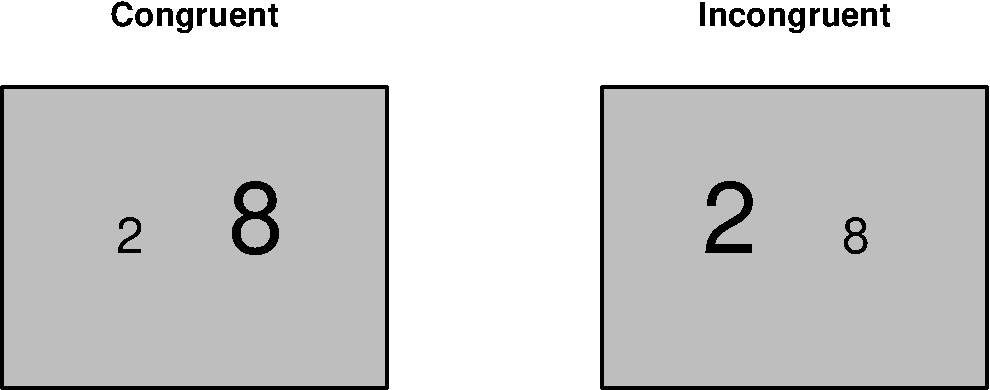
\includegraphics{paper_files/figure-latex/sceFigure-1.pdf}
\caption{\label{fig:sceFigure}Example stimuli in a physical size comparison
task. The left panel depicts a congruent trial, where the physically
larger digit (8) is also the numerically larger digit. The right panel
depicts an incongruent trial, where the physically larger digit (2) is
the numerically smaller one.}
\end{figure}

Though it is itself a curious result, the size-congruity effect may
perhaps be more important for the subsequent debate it has generated
concerning the nature of number representation. According to one
theoretical account, the size-congruity effect occurs because a digit's
physical size and numerical magnitude are both encoded into a common,
analog represention, upon which further processing occurs in a serial
fashion. This \emph{early interaction} account (Reike \& Schwarz, 2017;
Schwarz \& Heinze, 1998; Szűcs \& Soltész, 2007, 2008) predicts that the
relative slowdown on incongruent trials is due to interference at the
\emph{encoding} stage.

An alternative account posits that physical size and numerical magnitude
are encoded separately along independent pathways, and the interference
between physical size and numerical magnitude occurs as competition
between parallel and partially active response options (Faulkenberry et
al., 2016; Santens \& Verguts, 2011). In contrast to the early
interaction account, this \emph{late interaction} account predicts that
the locus of the size-congruity effect is not in the encoding stage, but
rather in the \emph{decision} stage.

A variety of paradigms have been employed to test between these
competing models of the size-congruity effect, including classical
response time (RT) tasks (Henik \& Tzelgov, 1982), electrophysiological
techniques (Schwarz \& Heinze, 1998; Szűcs \& Soltész, 2007, 2008),
neuroimaging (R. Cohen Kadosh et al., 2007), computer mouse tracking
(Faulkenberry et al., 2016), and visual search (Krause, Bekkering,
Pratt, \& Lindemann, 2016; Sobel, Puri, \& Faulkenberry, 2016; Sobel,
Puri, Faulkenberry, \& Dague, 2017). However, the evidence is quite
mixed, and as such, a clear consensus on the origin of the
size-congruity effect remains elusive.

A potentially fruitful method for elucidating the nature of the
size-congruity effect may come from employing \emph{accumulator models}
to describe the \emph{distributions} of RTs that are produced in the
comparison task. Generally speaking, an accumulator model posits that
responses in decision tasks stem from a process that involves noisy
accumulation of stimulus information over time. When the accumulated
information reaches a certain threshold, a response is initiated. An
advantage of using an accumulator model for modeling RTs is that by
fitting such a model, one obtains estimates of distributional parameters
that can directly index the underlying cognitive processes involved in
the decision, such as the rate of information accumulation, the response
threshold, and the duration of non-decision processes including encoding
and response production (Anders, Alario, \& Maanen, 2016). Further,
these models are quite good at describing the shape of typical RT
distributions, which tend to be positively skewed (Luce, 1986). From a
measurement standpoint, this allows one to model the effects of
experimental manipulations on the \emph{entire distribution} of RTs,
rather than simply modeling the effects of manipulations on the
collapsed means or medians. The use of accumulator models has a rich
history in the behavioral sciences (Link \& Heath, 1975; Luce, 1986;
Ratcliff \& McKoon, 2008; Ratcliff, Smith, Brown, \& McKoon, 2016).
However, the use of such models has been relatively limited in the
context of numerical cognition.

Whereas some accumulator models have been quite well studied in the
context of two-choice decision tasks, such as the drift diffusion model
(Ratcliff et al., 2016) and the linear ballistic accumulator model
(Brown \& Heathcote, 2008; Heathcote \& Hayes, 2012), such models are
typically best suited for tasks in which the error rate is sufficiently
large (Anders et al., 2016). As a consequence, these models are
difficult to fit in tasks with very low error rates, such as the ones
typically employed in the context of single-digit symbolic number
representations. An alternative to the drift diffusion and linear
ballistic accumulator models is the \emph{shifted Wald model} (Anders et
al., 2016; Schwarz, 2001). The shifted Wald model is a
\emph{single}-boundary accumulator model whose probability density
represents the distribution of first-passage times of a continuous
diffusion process that drifts (with rate \(\gamma\)) toward a single
boundary of height \(\alpha\). Mathematically, the probability density
is given by

\[
f(x \mid \gamma,\alpha,\theta) = \frac{\alpha}{\sqrt{2\pi(x-\theta)^3}}\cdot \exp\Biggl(-\frac{(\alpha-\gamma(x-\theta))^2}{2(x-\theta)}\Biggr)
\] where \(x>0\) represents a specific data point (i.e., a single
response time), \(\gamma\) is the \emph{drift rate}, \(\alpha\) is the
\emph{response threshold}, and \(\theta\) is a rightward shift of the
entire distribution that represents \emph{nondecision time}.
Descriptively, each parameter characterizes a specific characteristic of
the distribution's appearance. This can be seen in Figure
\ref{fig:swParameters}, which depicts the effect of selectively
increasing each shifted Wald parameter. Increasing drift rate \(\gamma\)
results in a \enquote{spreading out} of the distribution, but leaves the
mode relatively stable. Increasing response threshold \(\alpha\)
increases variance to a lesser extent than does an increase of
\(\gamma\), but the mode is shifted quite substantially rightward.
Increasing nondecision time \(\theta\) does not change the variance, but
instead results in a pure \enquote{shift} of the distribution rightward.

\begin{figure}
\centering
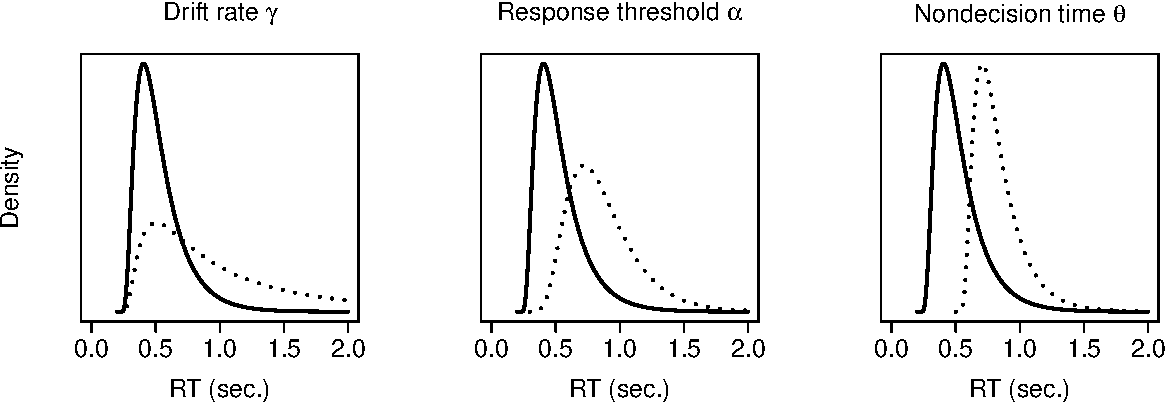
\includegraphics{paper_files/figure-latex/swParameters-1.pdf}
\caption{\label{fig:swParameters}Effects of manipulating shifted Wald (SW)
parameters on the shape of distributions. In all three plots, the solid
line depicts a SW density with drift rate = 3, response threshold = 1,
and nondecision time = 0.2 sec.~The dotted line depicts the resulting
density when exactly one of the parameters gets increased.}
\end{figure}

An important consideration for the present study is that each of the
three shifted Wald parameters can be interpreted as an index of specific
cognitive processes (Anders et al., 2016; Heathcote, 2004; Schwarz,
2001). Specifically, drift rate \(\gamma\) indexes rate of information
uptake from stimuli, response threshold \(\alpha\) indexes response
caution (that is, the amount of accumulated information required before
initiating a response), and nondecision time \(\theta\) indexes
processes not related to the accumulation process, such as stimulus
encoding and response production. For example, Anders, Riès, Maanen, and
Alario (2015) fit RT distributions in a picture naming task and found
that greater semantic interference resulted in slower drift rate (i.e.,
slower information accumulation) and larger response threshold, but no
change in nondecision time. These effects on the shifted Wald parameters
were largely consistent with predictions of the \enquote{dark-side
model}, a model of lexical choice in psycholinguistics (Oppenheim, Dell,
\& Schwartz, 2010). Another example in the context of numerical
cognition comes from Faulkenberry (2017), who had participants complete
an addition verification task under varying problem formats (words or
digits). He found that presenting problems in word format resulted in a
decrease in drift rate, concluding that the effect of problem format is
not isolated to the encoding stage, but rather has a direct impact on
calculation processes as well. This result was interpreted as support
for an interactive model of mental arithmetic processing (Campbell \&
Clark, 1988; Campbell \& Epp, 2004).

Against this background, the aim of the present study is to use the
shifted Wald distribution as a model to permit a fine-grained
examination of the size-congruity effect. Instead of collapsing
participants' RT distributions to single-valued summary statistics
(e.g., means or medians) and examining the effect of physical-numerical
size congruity on these means/medians, we instead fit the distributions
to a shifted Wald distribution, which yields estimates of drift rate,
response threshold, and nondecision time in each experimental condition.
If the early interaction account is correct, one should expect the size
congruity effects to stem from the encoding stage, and thus, one should
see a congruity effect on our estimates of nondecision time. If, on the
other hand, the late interaction account is correct, the size congruity
effect should stem from decision processes, and thus, one should see
congruity effects on our estimates of drift rate and response threshold.

\section{Method}\label{method}

\subsection{Participants}\label{participants}

Twenty-three undergraduate psychology students participated in the
experiment for partial course credit. Informed consent was obtained from
all individuals who participated in the study.

\subsection{Stimuli and procedure}\label{stimuli-and-procedure}

The experiment was implemented via the OpenSesame software package
(Mathôt, Schreij, \& Theeuwes, 2011), which was run on a 20 inch iMac
computer with a screen resolution of 1680 x 1050 pixels. Participants
used a standard Dell keyboard for input. At the beginning of the
experiment, participants were told that they would be presented with
pairs of numbers, with each number being displayed in a different font
size. Furthermore, they were told to quickly and accurately indicate
(via a keypress) which digit was physically larger, pressing the
\enquote{A} key if the number on the left was larger, and pressing the
\enquote{L} key if the number on the right was larger.

The number pairs were constructed from the single-digit Arabic numerals
2, 3, 4, 5, 6, 7, and 8. Pairs were chosen in order to balance the
numerical distance between numerals. Ignoring order, there were 12
possible pairs of numbers: 2-3, 3-4, 4-5 (distance 1); 2-4, 3-5, 4-6
(distance 2); 2-5, 3-6, 4-7 (distance 3); 2-6, 3-7, 4-8 (distance 4).

The size-congruity manipulation was created by varying the font size of
each digit in the number pair. Specifically, the physically smaller
digit was presented in 28 point font, whereas the physically larger of
the pair was presented in 36 point font. This resulted in two different
congruity conditions -- \emph{congruent} trials, in which the
numerically larger digit was also physically larger, and
\emph{incongruent} trials, in which the numerically larger digit was
physically smaller. Each pair was also presented in two different
left-right orders and two different font configurations
(smaller/left;larger/right or smaller/right;larger/left). In all, this
resulted in \(12 \times 2 \times 2 \times 2 = 96\) experimental trials
per block.

Participants completed 4 blocks of these 96 experimental trials (384
trials total) in a single experimental session lasting approximately 20
minutes. Each experimental trial began with a fixation cross displayed
for 500 milliseconds, followed immediately by a pair of numbers. The
center of the leftmost number was positioned 300 pixels to the left of
the center of the screen, whereas the center of the rightmost number was
positioned 300 pixels to the right of center (resulting in a visual
angle between numbers of approximately 25 degrees). For each trial, the
number pair remained on the screen until a response was made. If the
response was correct, no feedback was given, and the next trial began
immediately. If the response was incorrect, a red \enquote{X} was
presented in the center of the screen for 1 second, after which the next
trial began.

\section{Results}\label{results}

Participants completed a total of 8832 experimental trials. We discarded
433 trials that contained an incorrect response (error rate = 4.90\%).
Further, we removed an additional 87 trials for which response time was
below three median absolute deviations (MAD) and above six MAD from the
overall median RT (median RT = 559 msec, MAD = 142.33 msec) (Leys, Ley,
Klein, Bernard, \& Licata, 2013). This cleaning procedure resulted in
retaining a total of 8312 trials (94.10\% of original trials) for
further analysis.

The general analysis plan throughout the paper is as follows. First,
each hypothesis test was computed as a traditional frequentist test
(specifically, a paired-samples \(t\)-test). Afterward, we performed a
default Bayesian \(t\)-test (Rouder, Speckman, Sun, Morey, \& Iverson,
2009) to obtain a \emph{Bayes factor}, a likelihood ratio which provides
a continuous measure of the extent to which the observed data is more
likely to have occurred under one hypothesis than another (Kass \&
Raftery, 1995). As such, the Bayes factor provides a direct index of our
relative belief in one of two competing hypotheses. Notationally,
\(B_{10}\) represents a Bayes factor for the alternative over the null,
whereas \(B_{01}\) represents a Bayes factor for the null over the
alternative. This approach is especially useful in the case of null
effects, which cannot be coherently argued for within a frequentist
framework (Wagenmakers, 2007). By combining both frequentist and
Bayesian procedures, we can combine the familiarity of the frequentist
approch with a Bayesian measure of evidential value that is provided by
our data.

\begin{figure}
\centering
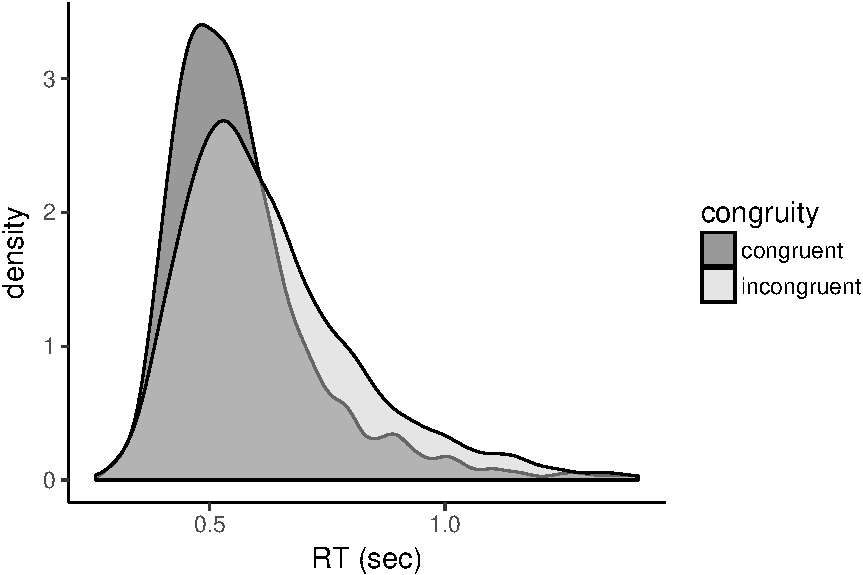
\includegraphics{paper_files/figure-latex/densities-1.pdf}
\caption{\label{fig:densities}Distributions of response times (in seconds)
as a function of congruity (congruent versus incongruent).}
\end{figure}

As expected, we found a significant size congruity effect on RTs in the
physical comparison task. As can be seen in Figure \ref{fig:densities},
the peak of the RT distribution for incongruent trials was shifted
rightward compared to the distribution for congruent trials, indicating
that incongruent trials took longer to compare than congruent trials.
This was confirmed by a paired samples \(t\)-test, from which we found a
signficant effect of congruity on median RTs, \(t(22) = 6.30\),
\(p < .001\). On average, responses for incongruent trials were 63
milliseconds slower than congruent trials. This result was well
supported by a Bayesian \(t\)-test, which produced a Bayes factor of
\(B_{10}=\) 15,679.05. This indicates that the observed data are
approximately 15679 times more likely under the alternative hypothesis
than the null hypothesis, which provides substantial evidence in favor
of a congruity-related increase in median RT.

Also apparent from Figure \ref{fig:densities} is an increase in the
spread of the RT distribution for incongruent trials. This was again
confirmed by a paired samples \(t\)-test: standard deviations were
signficantly larger for incongruent trials compared to congruent trials,
\(t(22) = 5.54\), \(p < .001\). Similar to median RTs, a Bayesian
\(t\)-test produced a Bayes factor of \(B_{10}=\) 3,152.15. As with
median RTs, this result implies that the observed data are approximately
3152 times more likely under the alternative than the null, giving us
much evidence in favor of a congruity-related increase in standard
deviations.

\begin{figure}
\centering
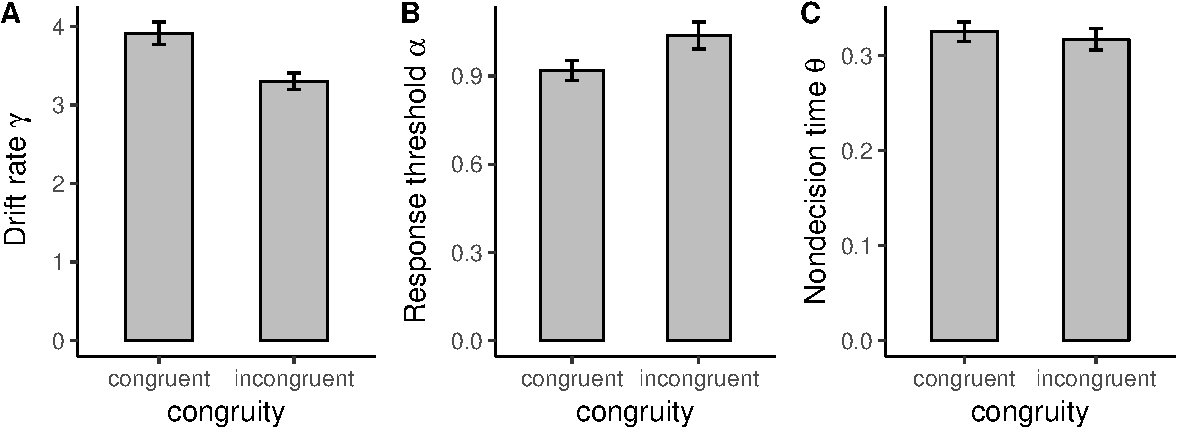
\includegraphics{paper_files/figure-latex/waldModel-1.pdf}
\caption{\label{fig:waldModel}Means of shifted Wald parameters presented as
a function of congruity (congruent versus incongruent). Panel A depicts
drift rate, which indexes rate of information accumulation from stimuli.
Panel B depicts response threshold, which indexes the amount of
accumulated information required before response initiation. Panel C
depicts nondecision time, which indexes the amount of time required for
nondecision processes (e.g., encoding and response generation).}
\end{figure}

Next, we attempted to more fully describe the effects of
physical-numerical size congruity on the \emph{distributions} of
response times. To this end, we fit the distributions with a shifted
Wald model. Specifically, each participant's distribution of RTs was
split into congruent trials and incongruent trials. Then, each of these
two distributions was fit with a shifted Wald model using the method of
Anders et al. (2016). This resulted in a collection of parameters
\(\gamma\) (drift rate), \(\alpha\) (response threshold), and \(\theta\)
(nondecision time) for each of the 46 combinations of congruity
(congruent, incongruent) and participant (\(N=\) 23). We then tested the
effects of congruity on the shifted Wald parameters by submitting each
parameter to a paired samples \(t\)-test. As above, we further validated
each result by measuring the evidential value of data in each test via a
Bayesian \(t\)-test.

The effects of physical-numerical size congruity on each shifted Wald
parameter can be seen in Figure \ref{fig:waldModel}. For drift rate
\(\gamma\), there was a significant effect of congruity,
\(t(22) = -5.27\), \(p < .001\). As can be seen in Figure
\ref{fig:waldModel}A, mean drift rate was smaller for incongruent trials
(\(M=\) 3.30) than for congruent trials (\(M=\) 3.91). This indicates
that the rate of information accumulation from incongruent trials was
reduced compared to trials in which the physical magnitude comparison
was congruent with the numerical magnitude comparison. A Bayesian
\(t\)-test yielded a Bayes factor of \(B_{10}=\) 1,729.35. This
indicates that the observed data are approximately 1729 times more
likely under the alternative hypothesis than the null hypothesis, which
provides very strong evidence in favor of a congruity-related decrease
in drift rate.

Figure \ref{fig:waldModel}B shows that congruity also had a significant
effect on response threshold \(\alpha\), albeit in the opposite
direction, \(t(22) = 3.15\), \(p = .002\). The mean response threshold
was larger for incongruent trials (\(M=\) 1.04) than for congruent
trials (\(M=\) 0.92), which indicates that in addition to a reduction in
the \emph{rate} of information accumulation on incongruent trials
compared to congruent trials, participants also required more
information before making a decision on such trials. A Bayesian
\(t\)-test resulted in a Bayes factor of \(B_{10}=\) 18.60, indicating
that the observed data are approximately 19 times more likely under the
alternative hypothesis than the null. Such a Bayes factor is generally
interpreted as positive evidence in favor of a congruity-related
increase in response threshold.

Finally, Figure \ref{fig:waldModel}C shows that congruity did not have a
significant effect on nondecision time \(\theta\), \(t(22) = -1.16\),
\(p = .870\). Note that in a frequentist framework, the absence of a
significant effect does not constitute evidence for a null effect
(Wagenmakers, 2007). We can, however, measure the evidence for a null
effect using a Bayes factor. To this end, a Bayesian \(t\)-test produced
a Bayes factor of \(B_{01}=\) 8.96, which means that the observed data
were approximately 9 times more likely under the null hypothesis than
the alternative hypothesis, giving us positive evidence in favor of a
null effect of congruity on nondecision time.

\section{Discussion}\label{discussion}

The purpose of the present study was to use response time modeling to
provide a fine-grained examination of the size congruity effect.
Specifically, we aimed to use the results of this modeling to test
between two competing models of the size congruity effect: an
\emph{early interaction} model, where the interference between physical
and numerical magnitude is purported to be an \emph{encoding} effect
which occurs an at early representational stage, and a \emph{late
interaction} model, where interference occurs at later,
\emph{decision}-related stages.

As was expected, we found a large effect of physical-numerical congruity
on median response times, which incongruent trials requiring
significantly more time for comparison than congruent trials. Further,
we found that the standard deviation of the response time distributions
increased for incongruent trials. Such an increase in both the center
and spread of the response time distributions indicates a need for more
fine-grained analysis of the effects of congruity on the response times
distributions. To this end, we used a shifted Wald distribution (Anders
et al., 2016), a single-boundary accumulator model, to provide a
three-parameter description of the distributions in each congruity
condition.

We found that congruent trials resulted in signficant changes to two of
the three shifted Wald parameters. The observed increase in median RT
and standard deviation that occured for incongruent trials was due
primarily to a decrease in drift rate and an increase in response
threshold. The decrease in drift rate means that, for incongruent
trials, stimulus information was accumulated more slowly than for
congruent trials. Simultaneously, there was an increase in response
threshold, indicating that participants adopted a larger threshold for
information that was required to be accumulated before making a
decision. Critically, there was no effect of congruity on nondecision
time. In all, the present data indicates that the congruity manipulation
had effects on decision-related parameters (drift rate and response
threshold) and no direct effect on the parameter related to encoding
(nondecision time). As such, the pattern of obesrved behavior lends
direct support to a \emph{late interaction} model of the size congruity
effect.

Such a conclusion is in general agreement with several other recent
studies on the locus of interference in the size congruity effect, which
have used a variety techniques ranging from visual search (Sobel et al.,
2016, 2017) to computer mousetracking (Faulkenberry et al., 2016). The
cumulative data from these studies lend converging evidence on the
late-interaction account of the size congruity effect. In turn, these
data further support to a response competition model of number
comparison put forth by Verguts and colleagues (Gevers, Verguts,
Reynvoet, Caessens, \& Fias, 2006; Verguts, Fias, \& Stevens, 2005).

The present study is also novel in its use of response time modeling in
the context of numerical cognition. Such models have been used
successfully in a variety of other domains, and their advantages have
been discussed previously.

In summary, the present data shows that the size congruity effect in
physical number comparison arises due to late, response-related decision
processes, and is not localized to an early encoding stage. As such, the
data lends support for a late-interaction account of the size congruity
effect.

\paragraph{Conflict of interest}\label{conflict-of-interest}

On behalf of all authors, the corresponding author states that there is
no conflict of interest.

\paragraph{Ethical approval}\label{ethical-approval}

All procedures performed in studies involving human participants were in
accordance with the ethical standards of the institutional and/or
national research committee and with the 1964 Helsinki declaration and
its later amendments or comparable ethical standards.

\paragraph{Informed consent}\label{informed-consent}

Informed consent was obtained from all individual participants included
in the study.

\newpage

\section{References}\label{references}

\setlength{\parindent}{-0.5in} \setlength{\leftskip}{0.5in}

\hypertarget{refs}{}
\hypertarget{ref-anders2016}{}
Anders, R., Alario, F.-X., \& Maanen, L. V. (2016). The shifted Wald
distribution for response time data analysis. \emph{Psychological
Methods}, \emph{21}(3), 309--327.
doi:\href{https://doi.org/10.1037/met0000066}{10.1037/met0000066}

\hypertarget{ref-anders2015}{}
Anders, R., Riès, S., Maanen, L. van, \& Alario, F.-X. (2015). Evidence
accumulation as a model for lexical selection. \emph{Cognitive
Psychology}, \emph{82}, 57--73.
doi:\href{https://doi.org/10.1016/j.cogpsych.2015.07.002}{10.1016/j.cogpsych.2015.07.002}

\hypertarget{ref-brown2008}{}
Brown, S. D., \& Heathcote, A. (2008). The simplest complete model of
choice response time: Linear ballistic accumulation. \emph{Cognitive
Psychology}, \emph{57}(3), 153--178.
doi:\href{https://doi.org/10.1016/j.cogpsych.2007.12.002}{10.1016/j.cogpsych.2007.12.002}

\hypertarget{ref-campbell1988}{}
Campbell, J. I. D., \& Clark, J. M. (1988). An encoding-complex view of
cognitive number processing: Comment on McCloskey, Sokol, and Goodman
(1986). \emph{Journal of Experimental Psychology: General},
\emph{117}(2), 204--214.
doi:\href{https://doi.org/10.1037/0096-3445.117.2.204}{10.1037/0096-3445.117.2.204}

\hypertarget{ref-campbell2004}{}
Campbell, J. I. D., \& Epp, L. J. (2004). An encoding-complex approach
to numerical cognition in Chinese-English bilinguals. \emph{Canadian
Journal of Experimental Psychology}, \emph{58}(4), 229--244.
doi:\href{https://doi.org/10.1037/h0087447}{10.1037/h0087447}

\hypertarget{ref-cantlon2006}{}
Cantlon, J. F., \& Brannon, E. M. (2006). Shared system for ordering
small and large numbers in monkeys and humans. \emph{Psychological
Science}, \emph{17}(5), 401--406.
doi:\href{https://doi.org/10.1111/j.1467-9280.2006.01719.x}{10.1111/j.1467-9280.2006.01719.x}

\hypertarget{ref-cohenKadosh2007}{}
Cohen Kadosh, R., Cohen Kadosh, K., Linden, D. E. J., Gevers, W.,
Berger, A., \& Henik, A. (2007). The brain locus of interaction between
number and size: A combined functional magnetic resonance imaging and
event-related potential study. \emph{Journal of Cognitive Neuroscience},
\emph{19}(6), 957--970.
doi:\href{https://doi.org/10.1162/jocn.2007.19.6.957}{10.1162/jocn.2007.19.6.957}

\hypertarget{ref-faulkenberry2017}{}
Faulkenberry, T. J. (2017). A single-boundary accumulator model of
response times in an addition verification task. \emph{Frontiers in
Psychology}, \emph{8}.
doi:\href{https://doi.org/10.3389/fpsyg.2017.01225}{10.3389/fpsyg.2017.01225}

\hypertarget{ref-faulkenberryShaki2016}{}
Faulkenberry, T. J., Cruise, A., Lavro, D., \& Shaki, S. (2016).
Response trajectories capture the continuous dynamics of the size
congruity effect. \emph{Acta Psychologica}, \emph{163}, 114--123.
doi:\href{https://doi.org/10.1016/j.actpsy.2015.11.010}{10.1016/j.actpsy.2015.11.010}

\hypertarget{ref-gevers2006}{}
Gevers, W., Verguts, T., Reynvoet, B., Caessens, B., \& Fias, W. (2006).
Numbers and space: A computational model of the SNARC effect.
\emph{Journal of Experimental Psychology: Human Perception and
Performance}, \emph{32}(1), 32--44.
doi:\href{https://doi.org/10.1037/0096-1523.32.1.32}{10.1037/0096-1523.32.1.32}

\hypertarget{ref-heathcote2004}{}
Heathcote, A. (2004). Fitting Wald and ex-Wald distributions to response
time data: An example using functions for the S-PLUS package.
\emph{Behavior Research Methods, Instruments, \& Computers},
\emph{36}(4), 678--694.
doi:\href{https://doi.org/10.3758/bf03206550}{10.3758/bf03206550}

\hypertarget{ref-heathcote2012}{}
Heathcote, A., \& Hayes, B. (2012). Diffusion versus linear ballistic
accumulation: Different models for response time with different
conclusions about psychological mechanisms? \emph{Canadian Journal of
Experimental Psychology}, \emph{66}(2), 125--136.
doi:\href{https://doi.org/10.1037/a0028189}{10.1037/a0028189}

\hypertarget{ref-henik1982}{}
Henik, A., \& Tzelgov, J. (1982). Is three greater than five: The
relation between physical and semantic size in comparison tasks.
\emph{Memory \& Cognition}, \emph{10}(4), 389--395.
doi:\href{https://doi.org/10.3758/bf03202431}{10.3758/bf03202431}

\hypertarget{ref-kass1995}{}
Kass, R. E., \& Raftery, A. E. (1995). Bayes factors. \emph{Journal of
the American Statistical Association}, \emph{90}(430), 773.
doi:\href{https://doi.org/10.2307/2291091}{10.2307/2291091}

\hypertarget{ref-krause2016}{}
Krause, F., Bekkering, H., Pratt, J., \& Lindemann, O. (2016).
Interaction between numbers and size during visual search.
\emph{Psychological Research}, \emph{81}(3), 664--677.
doi:\href{https://doi.org/10.1007/s00426-016-0771-4}{10.1007/s00426-016-0771-4}

\hypertarget{ref-leys2013}{}
Leys, C., Ley, C., Klein, O., Bernard, P., \& Licata, L. (2013).
Detecting outliers: Do not use standard deviation around the mean, use
absolute deviation around the median. \emph{Journal of Experimental
Social Psychology}, \emph{49}(4), 764--766.
doi:\href{https://doi.org/10.1016/j.jesp.2013.03.013}{10.1016/j.jesp.2013.03.013}

\hypertarget{ref-link1975}{}
Link, S. W., \& Heath, R. A. (1975). A sequential theory of
psychological discrimination. \emph{Psychometrika}, \emph{40}(1),
77--105.
doi:\href{https://doi.org/10.1007/bf02291481}{10.1007/bf02291481}

\hypertarget{ref-luce1986}{}
Luce, R. D. (1986). \emph{Response times: Their role in inferring
elementary mental organization}. New York: Oxford University Press.

\hypertarget{ref-opensesame}{}
Mathôt, S., Schreij, D., \& Theeuwes, J. (2011). OpenSesame: An
open-source, graphical experiment builder for the social sciences.
\emph{Behavior Research Methods}, \emph{44}(2), 314--324.
doi:\href{https://doi.org/10.3758/s13428-011-0168-7}{10.3758/s13428-011-0168-7}

\hypertarget{ref-oppenheim2010}{}
Oppenheim, G. M., Dell, G. S., \& Schwartz, M. F. (2010). The dark side
of incremental learning: A model of cumulative semantic interference
during lexical access in speech production. \emph{Cognition},
\emph{114}(2), 227--252.
doi:\href{https://doi.org/10.1016/j.cognition.2009.09.007}{10.1016/j.cognition.2009.09.007}

\hypertarget{ref-pavio1975}{}
Paivio, A. (1975). Perceptual comparisons through the mind's eye.
\emph{Memory \& Cognition}, \emph{3}(6), 635--647.
doi:\href{https://doi.org/10.3758/bf03198229}{10.3758/bf03198229}

\hypertarget{ref-ratcliff2008}{}
Ratcliff, R., \& McKoon, G. (2008). The diffusion decision model: Theory
and data for two-choice decision tasks. \emph{Neural Computation},
\emph{20}(4), 873--922.
doi:\href{https://doi.org/10.1162/neco.2008.12-06-420}{10.1162/neco.2008.12-06-420}

\hypertarget{ref-ratcliff2016}{}
Ratcliff, R., Smith, P. L., Brown, S. D., \& McKoon, G. (2016).
Diffusion decision model: Current issues and history. \emph{Trends in
Cognitive Sciences}, \emph{20}(4), 260--281.
doi:\href{https://doi.org/10.1016/j.tics.2016.01.007}{10.1016/j.tics.2016.01.007}

\hypertarget{ref-reike2017}{}
Reike, D., \& Schwarz, W. (2017). Exploring the origin of the
number-size congruency effect: Sensitivity or response bias?
\emph{Attention, Perception, \& Psychophysics}, \emph{79}(2), 383--388.
doi:\href{https://doi.org/10.3758/s13414-016-1267-4}{10.3758/s13414-016-1267-4}

\hypertarget{ref-rouder2016}{}
Rouder, J. N. (2016). The what, why, and how of born-open data.
\emph{Behavioral Research Methods}, \emph{48}, 1062--1069.
doi:\href{https://doi.org/10.3758/s13428-015-0630-z}{10.3758/s13428-015-0630-z}

\hypertarget{ref-rouder2009}{}
Rouder, J. N., Speckman, P. L., Sun, D., Morey, R. D., \& Iverson, G.
(2009). Bayesian \(t\) tests for accepting and rejecting the null
hypothesis. \emph{Psychonomic Bulletin \& Review}, \emph{16}(2),
225--237.
doi:\href{https://doi.org/10.3758/pbr.16.2.225}{10.3758/pbr.16.2.225}

\hypertarget{ref-santens2011}{}
Santens, S., \& Verguts, T. (2011). The size congruity effect: Is bigger
always more? \emph{Cognition}, \emph{118}(1), 94--110.
doi:\href{https://doi.org/10.1016/j.cognition.2010.10.014}{10.1016/j.cognition.2010.10.014}

\hypertarget{ref-schwarz2001}{}
Schwarz, W. (2001). The ex-Wald distribution as a descriptive model of
response times. \emph{Behavior Research Methods, Instruments, \&
Computers}, \emph{33}(4), 457--469.
doi:\href{https://doi.org/10.3758/bf03195403}{10.3758/bf03195403}

\hypertarget{ref-schwarzHeinze1998}{}
Schwarz, W., \& Heinze, H. J. (1998). On the interaction of numerical
and size information in digit comparison: A behavioral and event-related
potential study. \emph{Neuropsychologia}, \emph{36}(11), 1167--1179.
doi:\href{https://doi.org/10.1016/s0028-3932(98)00001-3}{10.1016/s0028-3932(98)00001-3}

\hypertarget{ref-sobel2016}{}
Sobel, K. V., Puri, A. M., \& Faulkenberry, T. J. (2016). Bottom-up and
top-down attentional contributions to the size congruity effect.
\emph{Attention, Perception, \& Psychophysics}, \emph{78}(5),
1324--1336.
doi:\href{https://doi.org/10.3758/s13414-016-1098-3}{10.3758/s13414-016-1098-3}

\hypertarget{ref-sobel2017}{}
Sobel, K. V., Puri, A. M., Faulkenberry, T. J., \& Dague, T. D. (2017).
Visual search for conjunctions of physical and numerical size shows that
they are processed independently. \emph{Journal of Experimental
Psychology: Human Perception and Performance}, \emph{43}(3), 444--453.
doi:\href{https://doi.org/10.1037/xhp0000323}{10.1037/xhp0000323}

\hypertarget{ref-szucs2007}{}
Szűcs, D., \& Soltész, F. (2007). Event-related potentials dissociate
facilitation and interference effects in the numerical Stroop paradigm.
\emph{Neuropsychologia}, \emph{45}(14), 3190--3202.
doi:\href{https://doi.org/10.1016/j.neuropsychologia.2007.06.013}{10.1016/j.neuropsychologia.2007.06.013}

\hypertarget{ref-szucs2008}{}
Szűcs, D., \& Soltész, F. (2008). The interaction of task-relevant and
task-irrelevant stimulus features in the number/size congruency
paradigm: An ERP study. \emph{Brain Research}, \emph{1190}, 143--158.
doi:\href{https://doi.org/10.1016/j.brainres.2007.11.010}{10.1016/j.brainres.2007.11.010}

\hypertarget{ref-verguts2005}{}
Verguts, T., Fias, W., \& Stevens, M. (2005). A model of exact
small-number representation. \emph{Psychonomic Bulletin \& Review},
\emph{12}(1), 66--80.
doi:\href{https://doi.org/10.3758/bf03196349}{10.3758/bf03196349}

\hypertarget{ref-wagenmakers2007}{}
Wagenmakers, E.-J. (2007). A practical solution to the pervasive
problems of \(p\) values. \emph{Psychonomic Bulletin \& Review},
\emph{14}(5), 779--804.
doi:\href{https://doi.org/10.3758/bf03194105}{10.3758/bf03194105}






\end{document}
